\documentclass[12pt]{article}
\usepackage[paper = letterpaper, margin=1in]{geometry}

\usepackage{amsmath}
\usepackage[parfill]{parskip}
\usepackage{graphicx}
\usepackage{subcaption}
\usepackage{bold-extra}
\usepackage{listings}

\makeatletter
\renewcommand{\@seccntformat}[1]{}
\makeatother

\lstset{ 
	language=Java,
	showstringspaces=false,
	columns=flexible,
	basicstyle={\small\ttfamily},
	breaklines=true,
	breakatwhitespace=true,
	tabsize=3
}

\pagestyle{empty}
\begin{document}
	\vspace*{2em}
	
	\begin{center}
		{\LARGE \fontfamily{qpl}\selectfont\scshape\textbf{Project Phase 2}}
		
		{\large Botz\\}
		{\footnotesize Carl Yarwood, Garry Alcorn, Elisabeth Goggin}
	\end{center}
	
	\vspace*{2em}
	
	\section[Overview]{\Large\fontfamily{qpl}\selectfont\scshape Overview}
	
	The goal of this project was to create a program used AES and steganography to hide a message in an image file. We decided to use specifically PNG image files due to the fact we found them easier to work with than other image file types. Though we found examples of more complex forms of steganography during our research in the earlier phase of this project, we chose to use a more straightforward method of steganography due to its ease of implementation. We decided that we did not wish to deal with the headache that came from messing with moving images, whether they be videos or a moving image file type like for example a GIF.
	
	Interestingly, while working on our project, we found a lot of similarities between the methods we used and the methods used for corporate level watermarking. The method we used involved calculating the binary before anding it with a mask to encode the selected number of least significant bits.
	
	The name of our program, BaldMan comes from our research in the earlier phase where we found references to an early story of steganography involving a slave getting the message tattooed on his head and then growing his hair out before being shaved for the message's delivery.
	
	\subsection[Challenges Faced]{\hspace*{1em}\large\fontfamily{qpl}\selectfont\scshape Challenges Faced}
	
	The largest challenge we faced when deciding out how to implement image steganography was figuring out what on the byte level of the images we could mess with. For example, avoiding control bits and such. We luckily managed to find a java class that would extract the image's info without touching the other stuff. Ultimately, we found it was much easier to put the message or image into the disguising image than to pull it out.
	
	\section[Test Cases]{\Large\fontfamily{qpl}\selectfont\scshape Test Cases}
	
	In the following example we will be hiding Figure 1a inside Figure 1b to get an output of Figure 1c.
	\begin{figure}[h]
		\centering
		\begin{subfigure}[t]{0.3\textwidth}
			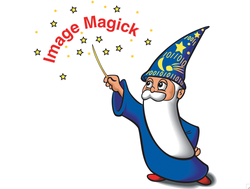
\includegraphics[width=\textwidth]{image/littleWizzard.png}
			\caption{The image to be hidden.}
		\end{subfigure}
		~
		\begin{subfigure}[t]{0.3\textwidth}
			
\includegraphics[width=\textwidth]{image/red.png}
			\caption{The image to hide the other image in.}
		\end{subfigure}
		~
		\begin{subfigure}[t]{0.3\textwidth}
			
\includegraphics[width=\textwidth]{image/newRed.png}
			\caption{The output in which the image is hidden.}
		\end{subfigure}
		\caption{Example images}
	\end{figure}
	
	\begin{figure}[h]
		\centering
		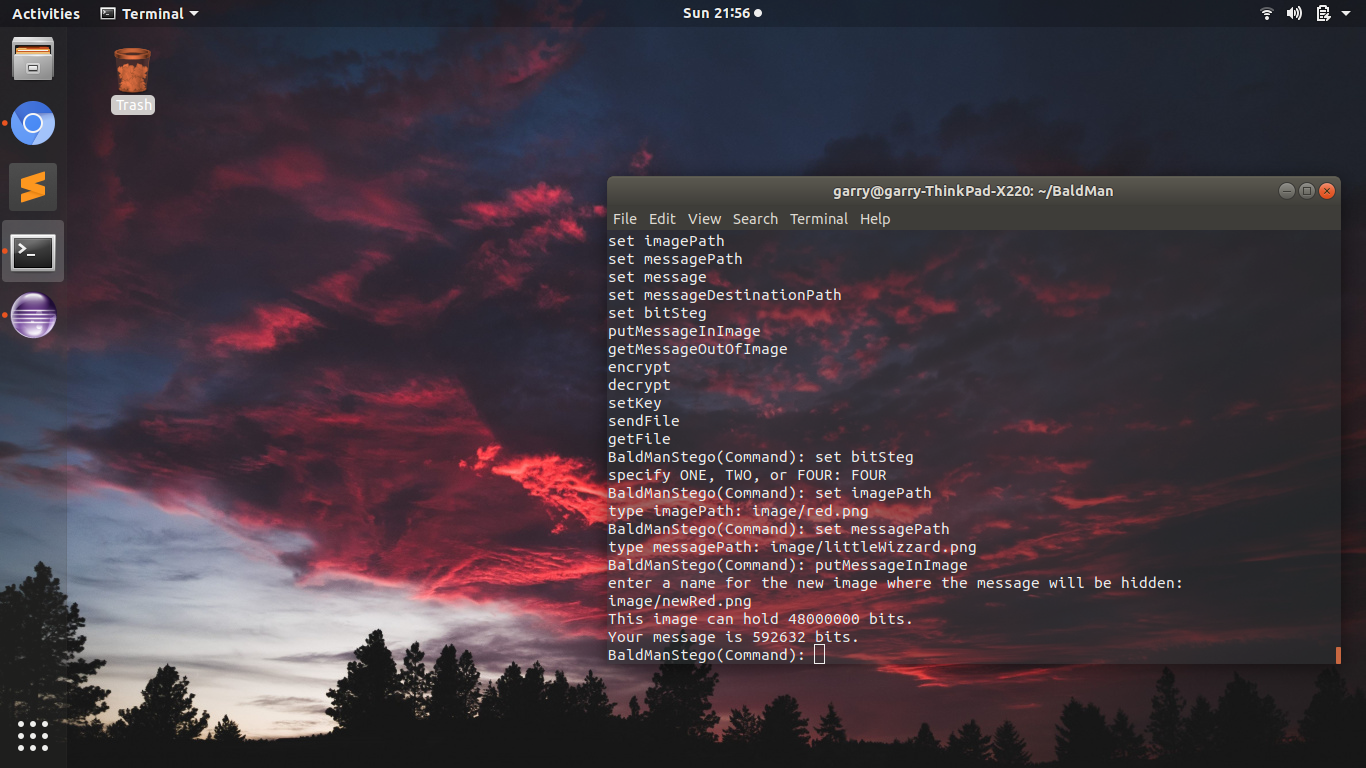
\includegraphics[keepaspectratio=true, width=0.8\linewidth]{screenshot.png}
		\caption{BaldMan running.}
	\end{figure}
	
	\begin{figure}[h]
		\centering
		
\includegraphics[keepaspectratio=true, width=0.8\linewidth]{image/bloob.png}
		\caption{This is an example of inserting too large of a message file into the image file causing distortion of the original image.}
	\end{figure}
	
	
	\section[Discussion]{\Large\fontfamily{qpl}\selectfont\scshape Discussion}
	
	\subsection[Max Bytes]{\hspace*{1em}\large\fontfamily{qpl}\selectfont\scshape Max Bytes}
	
	\section[Source Code]{\Large\fontfamily{qpl}\selectfont\scshape Source Code}
	
	\subsection[AESEncryption]{\hspace*{1em}\large\fontfamily{qpl}\selectfont\scshape AESEncryption.java}
	\lstinputlisting[language=Java]{AESEncryption.java}
	
	\subsection[BaldMan]{\hspace*{1em}\large\fontfamily{qpl}\selectfont\scshape BaldMan.java}
	\lstinputlisting[language=Java]{BaldMan.java}
	
	\subsection[Bits]{\hspace*{1em}\large\fontfamily{qpl}\selectfont\scshape Bits.java}
	\lstinputlisting[language=Java]{Bits.java}
	
	\subsection[Main]{\hspace*{1em}\large\fontfamily{qpl}\selectfont\scshape Main.java}
	\lstinputlisting[language=Java]{Main.java}
	
	\section[Project Contributions]{\Large\fontfamily{qpl}\selectfont\scshape Project Contributions}
	
	\begin{center}
		{\scshape\small
		\begin{tabular}{r l}
			\bfseries Research/Brainstorming & Carl Yarwood\\
			& Garry Alcorn\\
			& Elisabeth Goggin\\
			\bfseries Coding & Carl Yarwood\\
			& Garry Alcorn\\
			\bfseries Writeup & Elisabeth Goggin\\
		\end{tabular}
		}
	\end{center}
	
\end{document}